\documentclass[tikz,border=10pt]{standalone}
\usepackage{amsmath}
\usetikzlibrary{arrows.meta, positioning, calc, decorations.pathreplacing}
\definecolor{c1}{HTML}{000000}
\definecolor{c2}{HTML}{233D4D}
\definecolor{c3}{HTML}{FE7F2D}
\definecolor{c4}{HTML}{EAECF0}
\definecolor{axiscolor}{HTML}{333333}
\definecolor{labelcolor}{HTML}{5F6B75}
\begin{document}
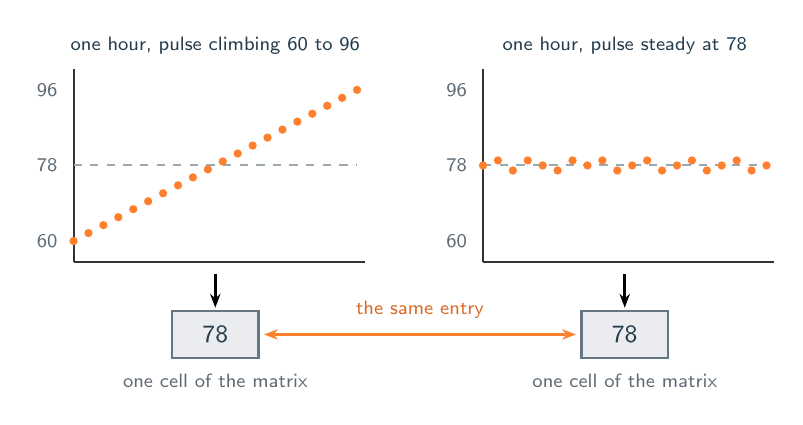
\begin{tikzpicture}[
    every node/.style={font=\sffamily},
    lab/.style={font=\sffamily\scriptsize, text=labelcolor},
    tag/.style={font=\sffamily\scriptsize, text=c2},
    arr/.style={-{Stealth[length=5pt]}, line width=1.0pt, color=c1},
    cell/.style={rectangle, draw=c2!70, fill=c4, line width=0.9pt,
                 minimum width=1.1cm, minimum height=0.6cm,
                 font=\sffamily\small, text=c2},
]
\def\Y#1{2.60 + (#1-55)*0.05333}

% ---------------- panel A: climbing
\node[tag] at (2.80, 5.35) {one hour, pulse climbing 60 to 96};
\draw[axiscolor, line width=0.7pt] (1.00, 2.60) -- (1.00, 5.05);
\draw[axiscolor, line width=0.7pt] (1.00, 2.60) -- (4.70, 2.60);
\node[lab, anchor=east] at (0.92, {\Y{60}}) {60};
\node[lab, anchor=east] at (0.92, {\Y{78}}) {78};
\node[lab, anchor=east] at (0.92, {\Y{96}}) {96};
\draw[c2!45, line width=0.7pt, dashed] (1.00, {\Y{78}}) -- (4.60, {\Y{78}});
\foreach \i in {0,...,19}{
    \pgfmathsetmacro\xx{1.00 + \i*0.1895}
    \pgfmathsetmacro\pp{60 + \i*1.895}
    \fill[c3] (\xx, {\Y{\pp}}) circle (1.5pt);
}

% ---------------- panel B: flat
\node[tag] at (8.00, 5.35) {one hour, pulse steady at 78};
\draw[axiscolor, line width=0.7pt] (6.20, 2.60) -- (6.20, 5.05);
\draw[axiscolor, line width=0.7pt] (6.20, 2.60) -- (9.90, 2.60);
\node[lab, anchor=east] at (6.12, {\Y{60}}) {60};
\node[lab, anchor=east] at (6.12, {\Y{78}}) {78};
\node[lab, anchor=east] at (6.12, {\Y{96}}) {96};
\draw[c2!45, line width=0.7pt, dashed] (6.20, {\Y{78}}) -- (9.80, {\Y{78}});
\foreach \i/\j in {0/0,1/1,2/-1,3/1,4/0,5/-1,6/1,7/0,8/1,9/-1,
                  10/0,11/1,12/-1,13/0,14/1,15/-1,16/0,17/1,18/-1,19/0}{
    \pgfmathsetmacro\xx{6.20 + \i*0.1895}
    \pgfmathsetmacro\pp{78 + \j*1.2}
    \fill[c3] (\xx, {\Y{\pp}}) circle (1.5pt);
}

% ---------------- the two cells
\draw[arr] (2.80, 2.45) -- (2.80, 2.02);
\draw[arr] (8.00, 2.45) -- (8.00, 2.02);
\node[cell] (a) at (2.80, 1.68) {78};
\node[cell] (b) at (8.00, 1.68) {78};
\node[lab, anchor=north] at (2.80, 1.30) {one cell of the matrix};
\node[lab, anchor=north] at (8.00, 1.30) {one cell of the matrix};

\draw[{Stealth[length=5pt]}-{Stealth[length=5pt]}, c3, line width=1.0pt]
    (3.42, 1.68) -- (7.38, 1.68);
\node[font=\sffamily\scriptsize, text=c3!85!black, anchor=south]
    at (5.40, 1.76) {the same entry};
\end{tikzpicture}
\end{document}
